\begin{flushright}
\emph{"With four parameters I can fit an elephant, and with five I can make him wiggle his trunk."}\\
— John von Neumann, circa 1953
\end{flushright}

\vspace{0.5em}


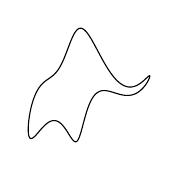
\begin{tikzpicture}[x=0.01cm,y=0.01cm]  
  \draw[smooth, domain=0:360, variable=\t, samples=400]
    plot
      ({-60*cos(\t) + 30*sin(\t) - 8*sin(2*\t) + 10*sin(3*\t)},
       { 50*sin(\t) + 18*sin(2*\t) - 12*cos(3*\t) + 14*cos(5*\t)});
\end{tikzpicture}
\vspace{0.5em}

\begin{flushright}
\emph{A curve found in 2010 as shown above.}\\
\emph{The curve can be fitted with four parameters. A fifth point can beadded to form the elephant's eye and allows the trunk to move.}
\\
— Jürgen Mayer, Khaled Khairy, Jonathon Howard, 2010
\end{flushright}
